\subsection{Functional Role}

The analysis of functional role covered by the java class under inspection would be quite superficial and with more arising questions than answers if a worthful overview of the most important elements of the project would not be taken in consideration.

Thus, before meeting the goal of this section, a glance to the relevant concept for our analysis is given.

\subsubsection{OFBIz overview}
The Open For Business project is an enterprise-oriented suite of applications developed to support most of the aspects that an enterprise application has to take care of.

The applications share the same underlying architecture, using common data, logic and process components.

A loosely coupled approach is used as base for the architecture, allowing an easy extension of the suite itself.

Each application is loosely coupled with the others, easing the updating and the extension.

\subsubsection{Entities and Services}
As stated by the official documentation:

\begin{itemize}
	\item \textbf{Entities}: an entity is a relational data construct that contains any number of Fields and can be related to other entities. Basic entities correspond to actual database structures.
	\item \textbf{Services}: a service is a simple process that performs a specific operation.
\end{itemize}

\subsubsection{Project's architecture}

The architecture of the entire suite is composed by 4 sets of components:

\begin{itemize}
	\item \textbf{Framework}
	\item \textbf{Applications}
	\item \textbf{Special Purpose}
	\item \textbf{Hot-deploy}
\end{itemize}

The sets of components, as well the contained components, are in a dependency relationship according to the dependency-arcs shown in the following diagram.

The dependency flow goes from top to bottom, either for component sets and for components.

This means that components and applications on the top are dependent on elements on the bottom of the same diagram. The viceversa should not be allowed.

The type of dependency may vary: foreign key dependency in the data model, application's service calling another application's service and so forth.

\begin{figure}[H]
	\centerline{
		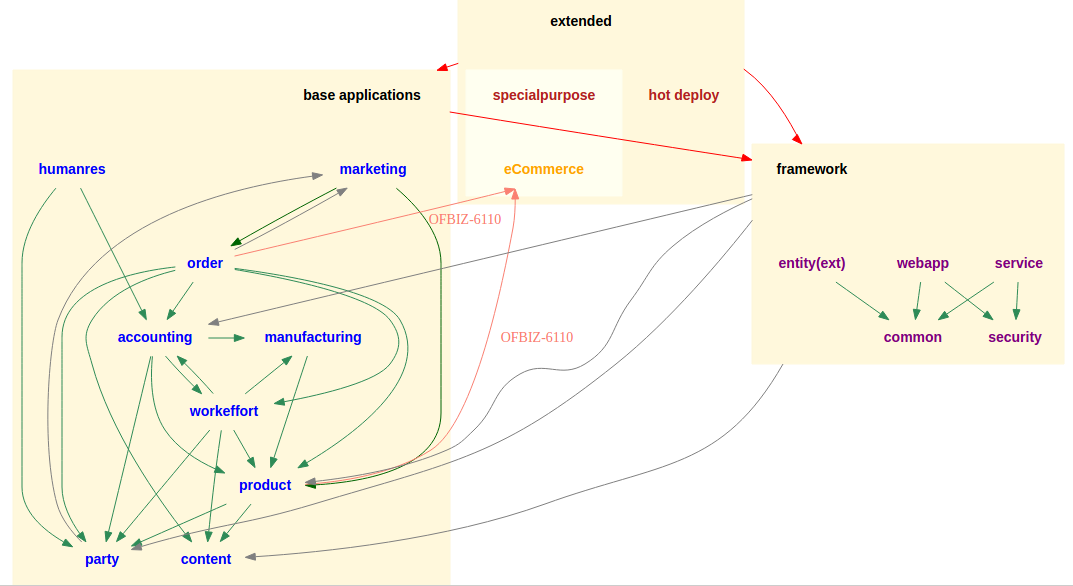
\includegraphics[width=350px]{../Datas/images/dependencies.png}
	}
	\label{fig:components-dependencies}
	\caption{Components dependencies}
\end{figure}

As can be seen, there's a relation of dependency between the human resource application and the party application.
\newpage

\subsubsection{Parties}
According to the {\textit{OFBIz project's overview}}\footnote{https://cwiki.apache.org/confluence/display/OFBIZ/Component+and+Component+Set+Dependencies}:

\textit{Party can be either a Person, or a group of Parties. A Party Group could be a company, an organization within the company, a supplier, a customer, and so forth.
Information that describes Parties or is directly related to Parties is contained in these entities.}

According to the party's data model, each party, either a person, a group and so forth, is identified by a unique ID number.

\subsubsection{Human Resource Entities}

According to the \textit{OFBIz project overview}:

\textit{The Human Resources entities are used to keep track of positions, responsibilities, skills, employment, termination, benefits, training, pay grades and payroll preferences, performance reviews, resumes and applications, and other Human Resources related information.}

\subsubsection{Internal Organization}
Quoting the \textit{human resource glossary}\footnote{https://cwiki.apache.org/confluence/display/OFBIZ/Human+Resources+Glossary}:

\textit{Internal organization is the name of a relationship between a party group and your company.}

\textit{This relationship is used to filter party groups as being part of your company to distinguish them from other groups which are external.}

\textit{For example your marketing department is an internal organization while a suppliers sales department is not.}

\subsubsection{Employee Position}

Also abbreviated as \textit{position}, it is an entity used to represent a work position inside the company.
Quoting the \textit{official documentation of the project}\footnote{https://cwiki.apache.org/confluence/display/OFBIZ/Employee+Position}:

\textit{In OFBiz a position is the authorization, typically from the budget of an internal organization, for the Company to engage one person to do a job. OFBiz handles positions in a flexible manner so you can think of a position as an authorization for a full-time equivalent (FTE).}

\textit{This means that you can fulfill a position with a person in a number of different ways. You can fill a position with one full time person, change the assignment of a position from one person to another over time, or split a position across more then one person at the same a time.}

\textit{As implemented a position can be fulfilled by \textbf{either a person or organization}.}

The data model\footnote{https://cwiki.apache.org/confluence/display/OFBIZ/Data+Model+Diagrams} representing a employee position is quite huge and complex, so only the essential part for our analysis are shown and described.

\textbf{NB:}\textit{The whole data model diagram on the wiki is not up to date, therefore there could be some discrepancy between it and the documentation.}

\begin{figure}[H]
	\centerline{
		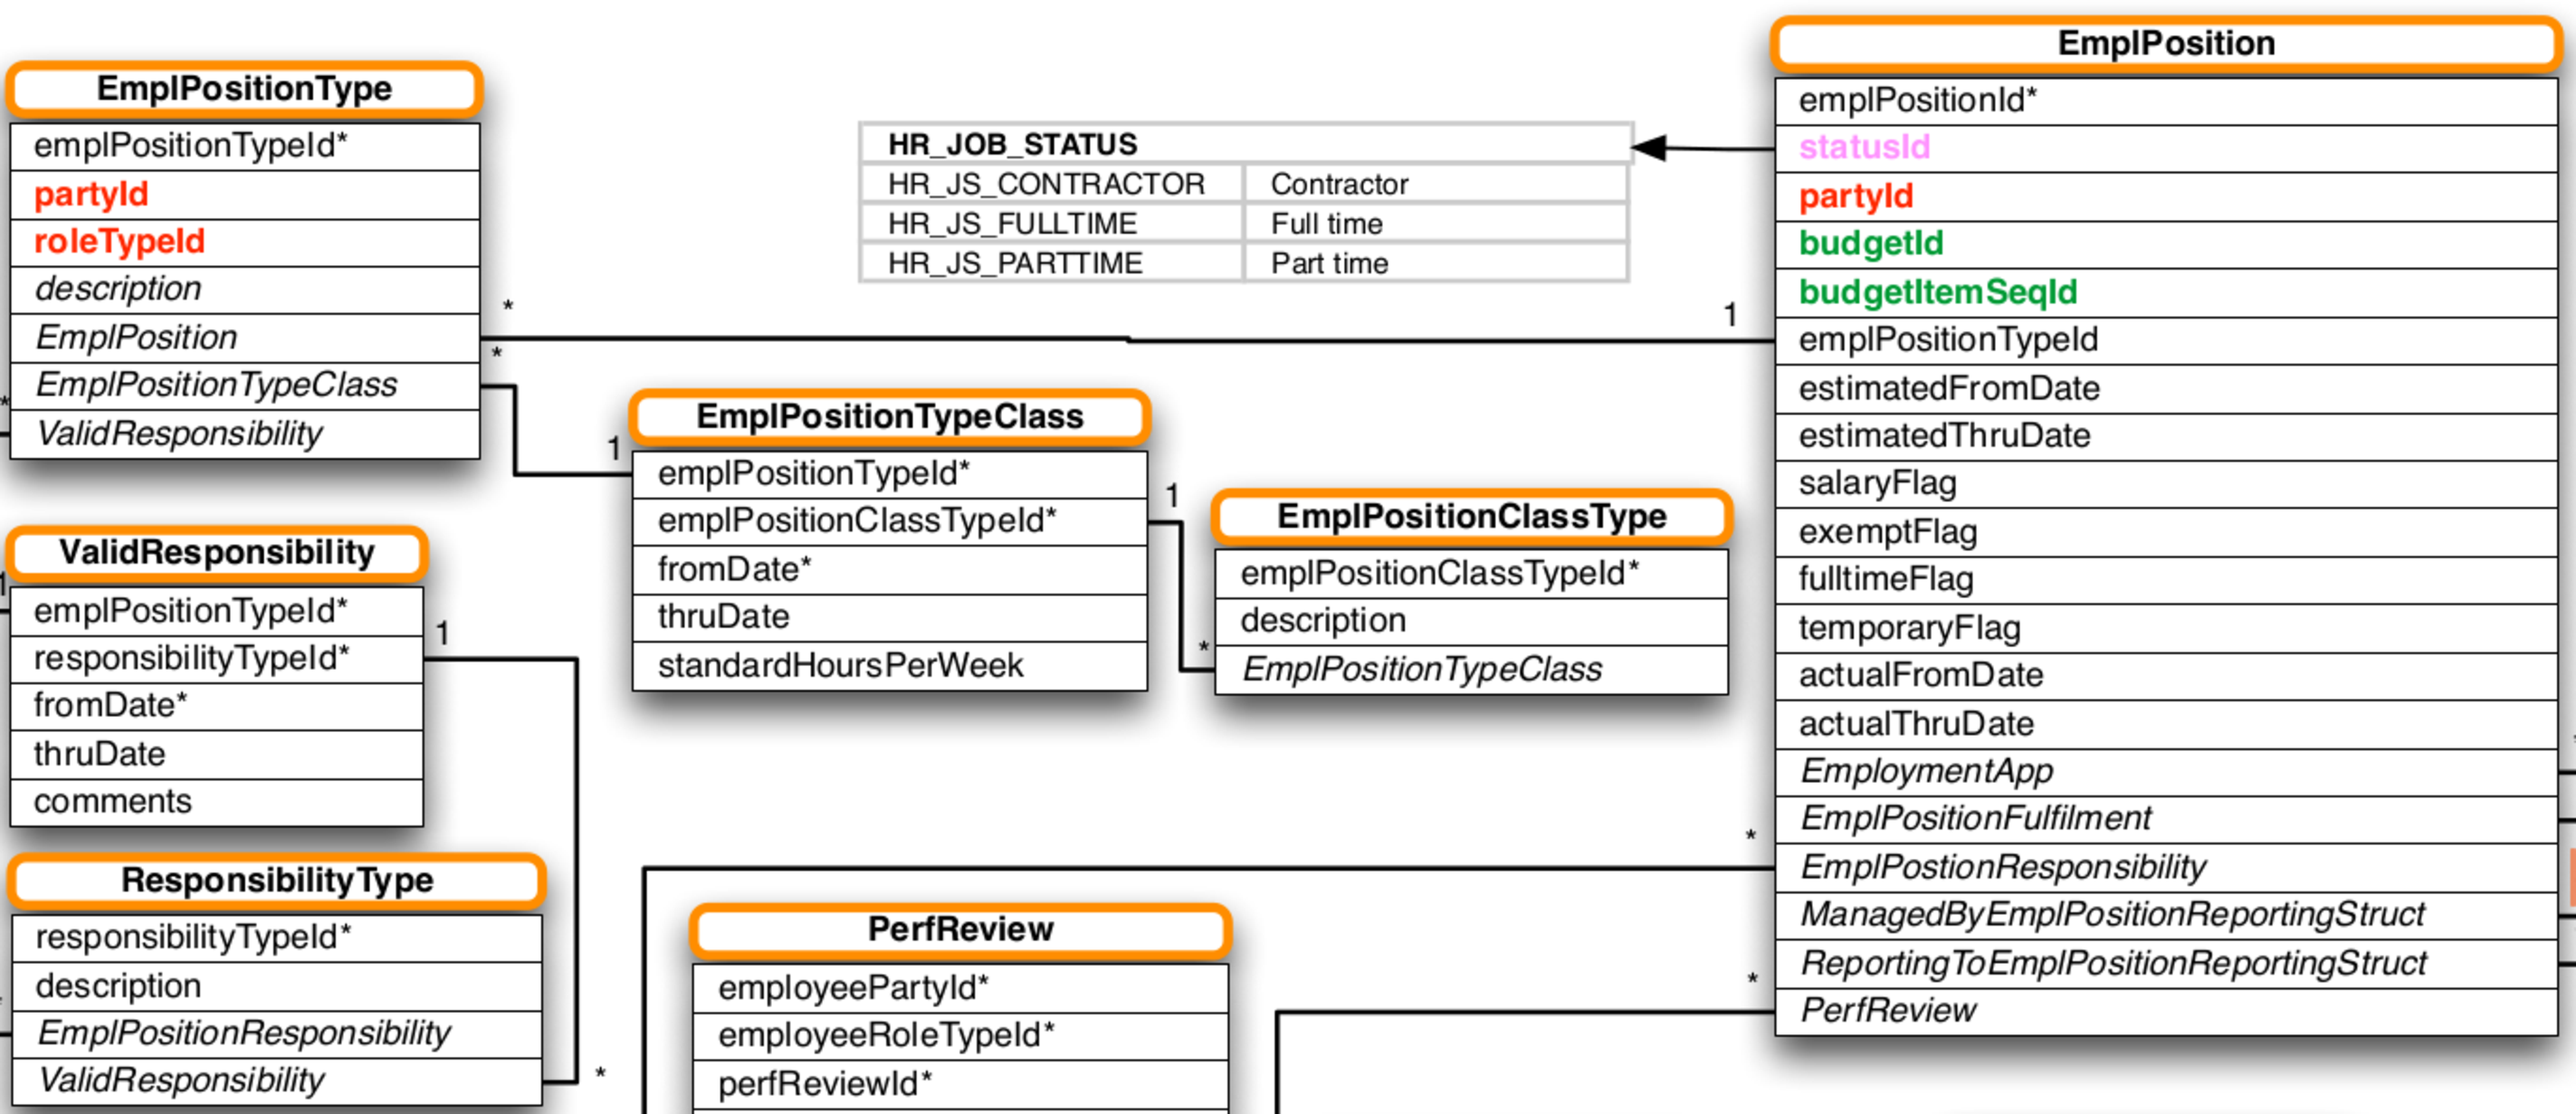
\includegraphics[width=350px]{../Datas/images/emplPos-posType.pdf}
	}
	\label{fig:emplPos-type}
	\caption{Employ Position - Employ Position Type relationship}
\end{figure}

\begin{itemize}
	\item \textbf{EmplPosition}: entity used to represent an employee position inside the Human Resource Application. 

	Each entity is characterized by several. The most relevant for our analysis are:


	\begin{itemize}
		\item \textbf{emplPositionId:} an \textbf{unique} identifier used to distinguish a position from another one.
		\item \textbf{statusId:} a string identifying the status of the position.

		Actually, the documentation and the data model of the emplPosition entity diverge about the content of this field. 

		The former specifies that it is used to state if the position is \textbf{Active/Open}, \textbf{Inactive/Closed} or \textbf{Planned for}, while the data model diagram report is as a field specifying the type of position: \textbf{full time}, \textbf{part time} or \textbf{contractor}.

		As stated previously, the data model is not updated, therefore we take as reference what described by the documentation.
		\item \textbf{partyId}: the ID of the \textbf{Internal Organization} authorized to fill the position.
	\end{itemize}

	\item \textbf{EmplPositionType:} entity representing a possible type for a position. An example of position type is the Business Analyst or the System Administrator.
	Relevat fields are:

	\begin{itemize}
		\item \textbf{emplPositionTypeId:} unique identifier used to discern between position types.
		\item \textbf{partyId:}
		\item \textbf{description:} a description of the type of position.
		\item \textbf{EmplPosition:} identifier of the employee position having this specific type. 
	\end{itemize}  
\end{itemize}

\begin{figure}[H]
	\centerline{
		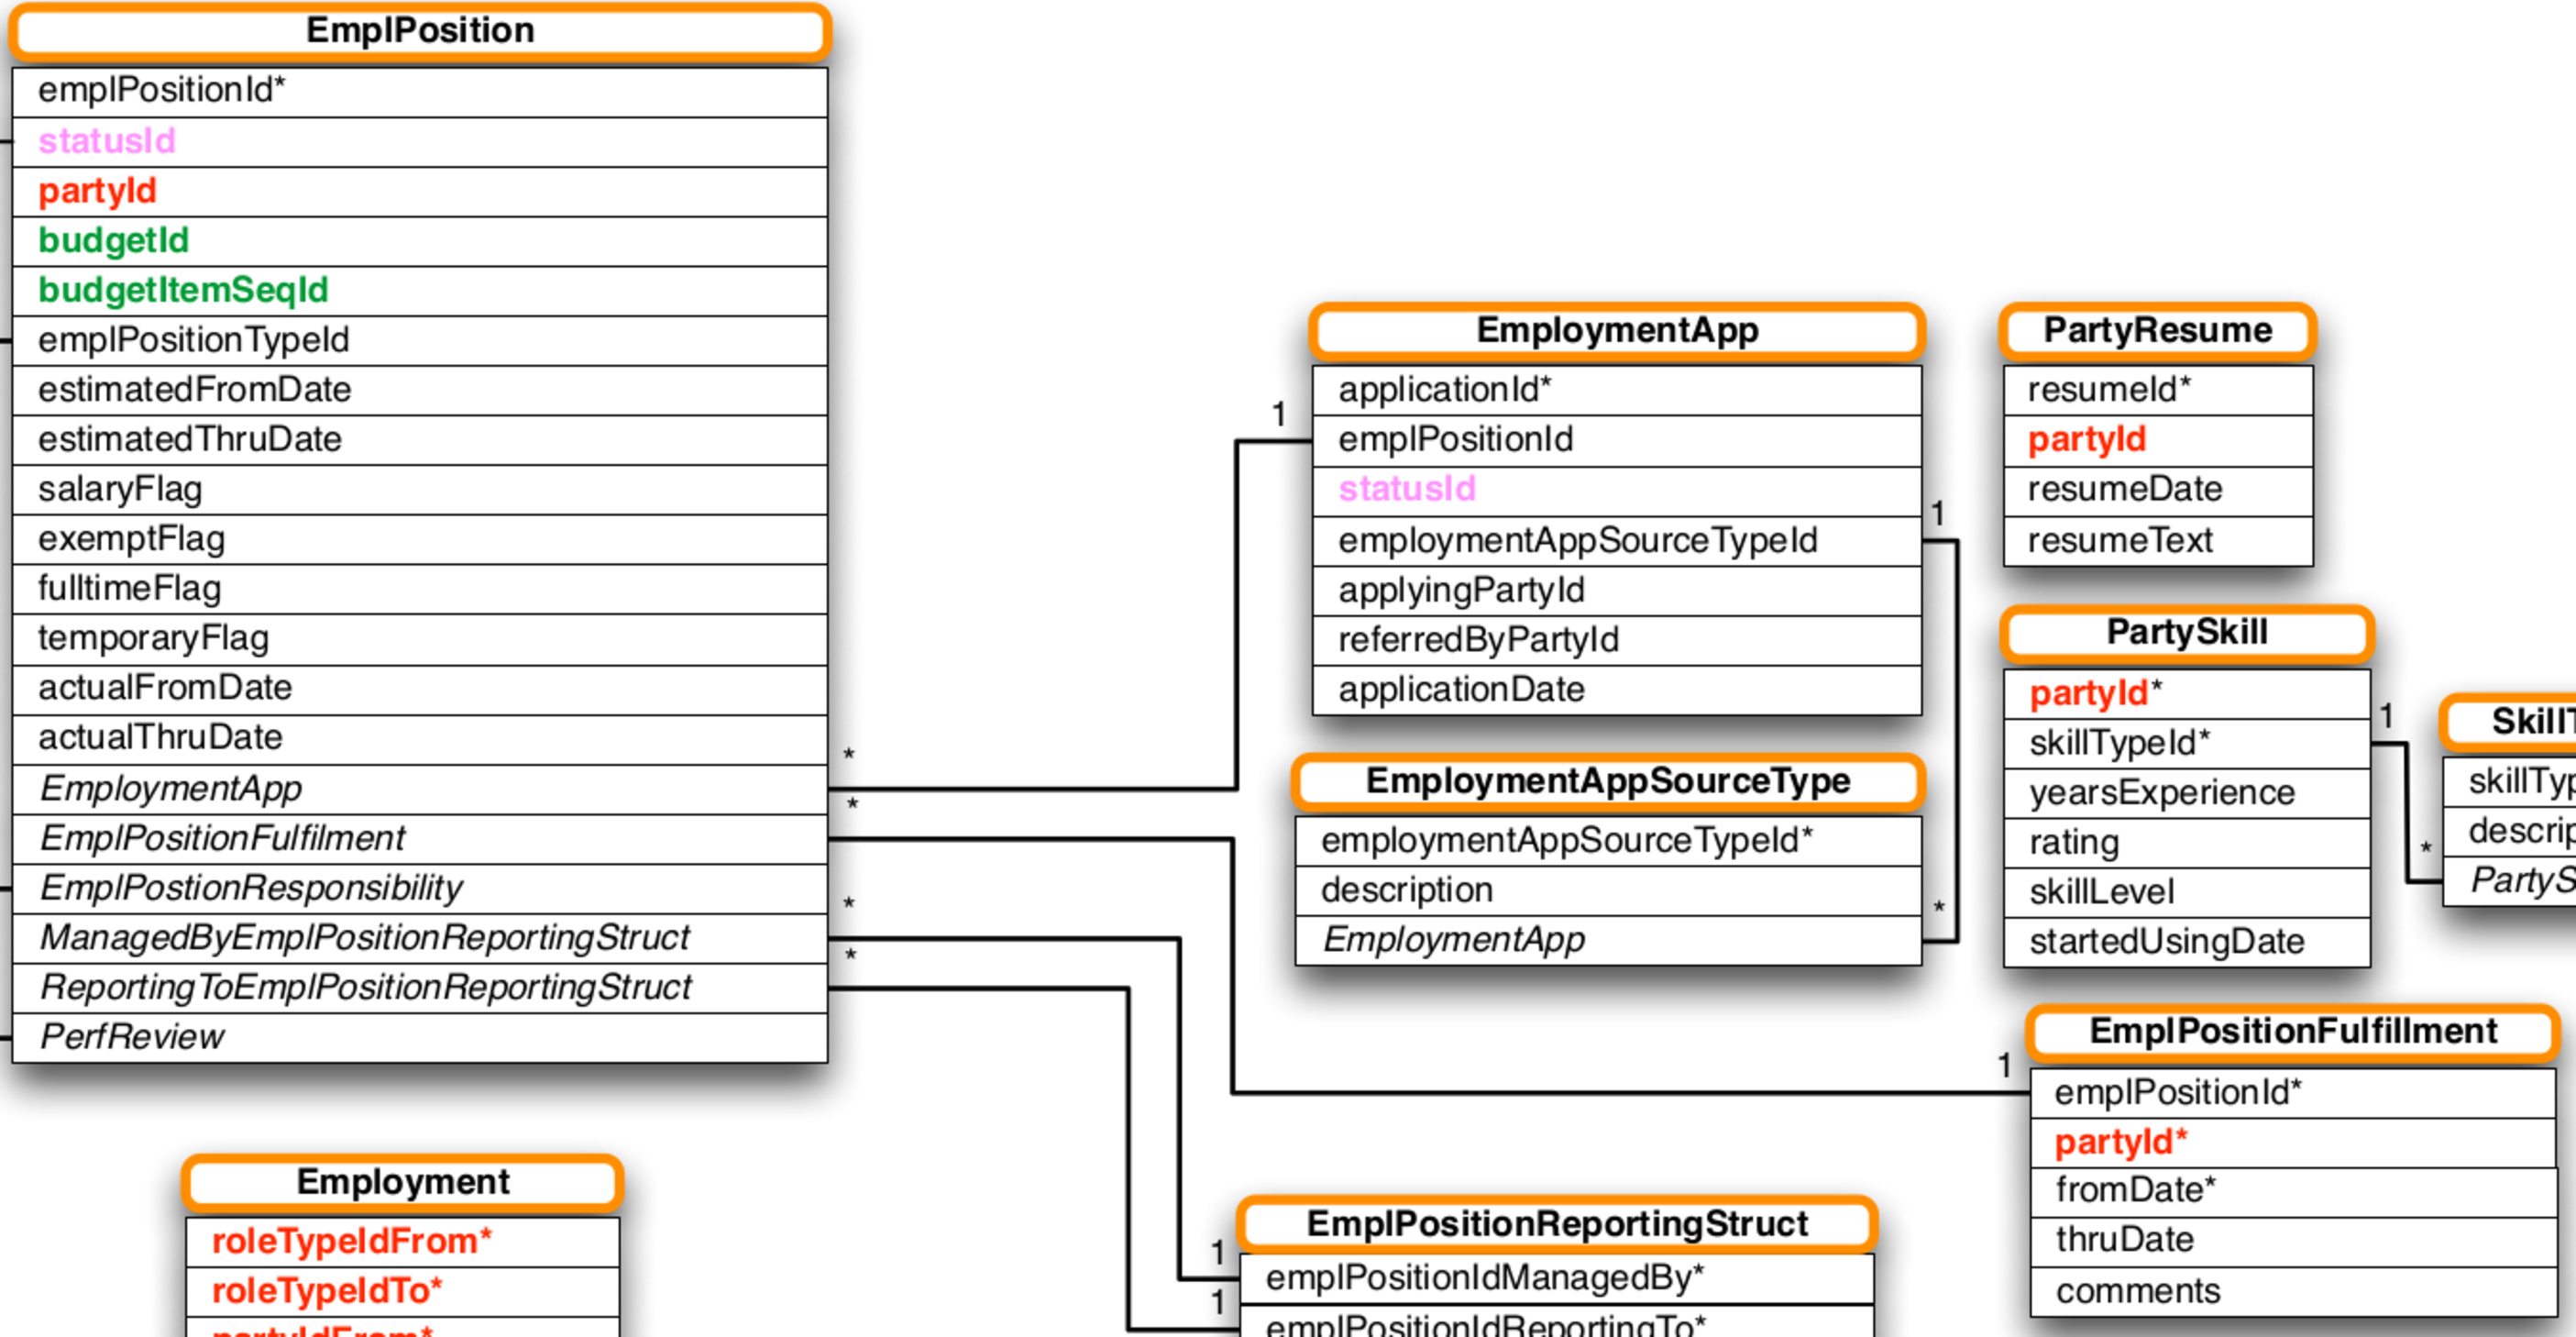
\includegraphics[width=350px]{../Datas/images/emplPos-fill.pdf}
	}
	\label{fig:emplPos-fill}
	\caption{Employee Position - Employee Position Fulfillment relationship}
\end{figure}

\begin{itemize}
	\item \textbf{EmplPositionFulfillment}: entity used to represent the party or parties that fulfill a specific position.
	Relevant informations of this entity are:

		\begin{itemize}
			\item \textbf{emplPositionId:} the ID of the position fulfilled by the party.
			\item \textbf{PartyId:} the ID of the party fulfilling the position.
			\item \textbf{fromDate:} the date from which the position is fulfilled.
		\end{itemize}
\end{itemize}

\subsubsection{Human resource application}

The human resource application comes with a predefined set of functionalities that can be used to perform HR tasks or to provide a support for the creation of more complex HR applications.\footnote{https://cwiki.apache.org/confluence/display/OFBIZ/Human+Resources+Guide} 

According to the documentation of the human Resources application\footnote{https://cwiki.apache.org/confluence/display/OFBIZ/Human+Resources+-+Main+Window}:

\textit{The Main window is the entry point into the Human Resources Application and displays the Company tree view for navigating to the main menu items.}

\textit{There are three node types in the tree, each identified by a different icon. The top of the tree represents your Company, the highest level in the organization. The Company and departments under the Company can have sub departments or positions. Under positions are the people who fulfill the position.}

Furthermore, as stated by the documentation, from the main screen of the application is possible:

\begin{itemize}
	\item Navigate the company hierarchy, viewing departements, position and people.
	\item Add or remove a department
	\item Add a person
	\item Quickly open the profile of any item in the tree
	\item If an item is a position, you can add a person to fulfill the position.
\end{itemize}

\subsubsection{Tree and HumanResEvents class}

In the previous paragraph the important role played by the tree has been discussed, showing how several important actions may be performed only through the tree itself. 

This tree is created each time the main screen of the human resources application is visited. The generation is performed thanks to a jquery script named \textit{createTree} and located in the \textit{humanres/template/category/CategoryTree.ftl} template file.
The script is executed each time the main screen is loaded, sending an asynchronous POST request to the resource located at \textit{getHRChild}.

According to the \textit{controller.xml} file, located in \textit{webapp/humanres/WEB-INF} folder, the \textit{getHRChild} resource is mapped to the only public method provided by the HumanResEvents class: \textbf{getChildHRCategoryTree}.

In the light of this premise and the concepts introduced before, it's quite easy and straigthforward understand the role of this class: help in the construction of the company tree by

\begin{itemize}
	\item Collecting the necessary informations of each party and position in the company.
	\item Using the collected informations to build the html attributes needed to enable the action performable through the tree (viewing departements, open profiles...).
\end{itemize}

The html attributes built for each party or position are returned in a \textbf{Map}, which structure follow the design of the json implementation of the tree, as stated by the comment on line 40.

As soon as the \textit{getChildHRCategoryTree} is invoked, the informations gathering begins. The driver is the \textbf{partyId} identificator passed as a parameter to the class method.

Since a company or a department may have positions or child departments, the public method manages the retriving of positions and child departments informations separatly.

The gathering of positions informations is performed invoking the \textit{getCurrentEmployeeDetails}, which queries the database about the presence of a employee position instance identified by the partyId identificator.

If positive, the computation goes on, verifying the presence of parties fulfilling that position. The check is made through a query against the \textit{EmplPositionFulfillment}.

In presence of parties fulfilling that position, the following informations are collected:

\begin{itemize}
	\item Name \& Surname of the employee.
	\item Group name of the departments and companies.
\end{itemize}

For each party, html attributes necessary to show the informations and create links to their profile are built and stored inside map structure.
After iterating over all the parties, the method ends and returns the list of map structures containing the informations of each party.

In both cases in which no employee position matches the partyId or no fulfillment is related to the position, the method ends returning an empty list.

\textbf{NB:} actually, the implementation of the \textit{getCurrentEmployeeDetails} provides the retrieving of informations of only one employee position, since each EmplPosition entity is identified by a unique identifier.

The retrieving of child departments informations is handled by two different methods.

The first one, \textit{getChildCompos}, retrieves the informations concerning the children of the partyGroup: querying the \textit{PartyRelationship} entity, it looks for parties that are in a father-child relationship with the partyGroup.

For each of the matching parties, the informations are retrieved and the html attributes built and stored in map structures, whichi are put in a list returned to the caller.

The informations are the same collected by the \textit{getCurrentEmployeeDetails}.

The second method, \textit{getChildInComp}, queries the \textit{EmplPosition} in order to find employee position currently active and authorized by the partyGroup. These informations are:

\begin{itemize}
	\item \textbf{emplPositionId:} the employee position identificator.
	\item \textbf{description:} description of the position type.
\end{itemize}

As always, the required html attributes are built and stored in map structures, in turn placed into a list returned to the caller
.

Maybe for an error, the comment preceding the invocation of this function in the public method states that it retrieves the informations of the employees working in the partyGroup, which is contrast with the behaviour of the method.

In the end, the \textit{getChildHRCategoryTree} method returns to the jquery script the concatenation of lists of maps created retrieving informations about positions and child departments.
 
